% File: basic_elements.tex
\documentclass{standalone}
\usepackage{pgfplots}
\pgfplotsset{compat=1.18}
\usepackage[american]{circuitikz}
\usepackage{cmbright}

\definecolor{myred}{RGB}{170,0,0}
\definecolor{myblue}{RGB}{0,0,220}

\ctikzset{bipoles/resistor/height=0.2}
\ctikzset{bipoles/resistor/width=0.5}


\begin{document}
% Simple RL circuit, with equations, and plots of different quantities.
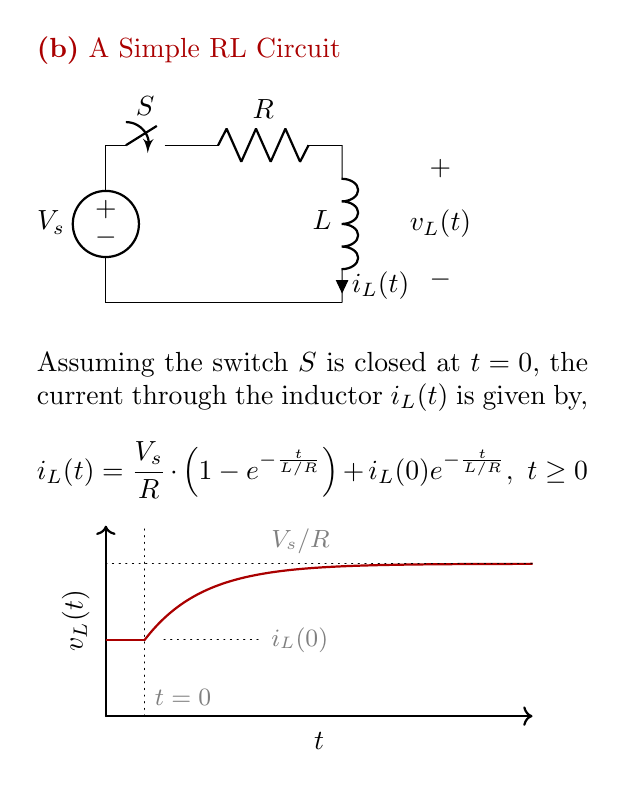
\begin{tikzpicture}
    % Subtitle for the circuit.
    \node[anchor=north west, color=myred] at (-1, 3.5) {\textbf{(b)} A Simple RL Circuit};
    % --- Circuit (top left)
    \begin{scope}
        % Coordinates.
        \coordinate (A) at (3, 2);
        \coordinate (B) at (3, 0);
        \coordinate (C) at (4.25, 2);
        \coordinate (D) at (4.25, 0);

        % Voltage source and lower wire
        \draw (0, 0) to[V, l={$V_{s}$}, invert] (0, 2) to[closing switch, l=$S$] ++(1, 0) to[R, l=$R$] (A);
        \draw (0, 0) -- (B);

        % Capacitor.
        \draw (A) to[L, l_=$L$, i^>=$i_L(t)$] (B);

        % Voltage label across A and B
        \draw (C) to[open, v^=$v_{L}(t)$] (D);
    \end{scope}

    % Plot of v_L vs i_L (top right)
    \begin{scope}[yshift=-0.5cm]
        % Subtitle for the circuit.
        \node[anchor=north west, color=black, text width=7cm, align=justify] at (-1, 0) {Assuming the switch $S$ is closed at $t=0$, the current through the inductor $i_L(t)$ is given by,
        \[ i_L(t) = \frac{V_s}{R} \cdot \left( 1 - e^{-\frac{t}{L/R}} \right) + i_L(0)e^{-\frac{t}{L/R}}, \,\, t\geq 0 \]
        };
    \end{scope}

    % Plot of i_L
    \begin{scope}[yshift=-5.25cm]
        \begin{axis}[
            width=7cm,
            height=4cm,
            xlabel={$t$},
            ylabel={$v_L(t)$},
            xmin=-1, xmax=10,
            ymin=0, ymax=2.5,
            samples=1000,
            domain=-1:10,
            thick,
            axis lines=left,
            axis line style={->},
            xtick=\empty,
            ytick=\empty,
            line cap=round
        ]
        % Constant value before t = 0
        \addplot[myred, thick, domain=-1:0] {1};
        % Exponential rise after t = 0 with final value 2, initial 1, tau = 1.5
        \addplot[myred, thick, domain=0:10] {2 - (2 - 1) * exp(-x/1.5)};
        \draw[dotted, thin, black] (axis cs:0,0) -- (axis cs:0,2.5);
        % Switch closing time
        \node[anchor=south west, color=gray] at (axis cs:0.0, 0.) {\small $t=0$};
        % Final voltage 
        \draw[dotted, thin, black] (axis cs:-1,2) -- (axis cs:10, 2);
        \node[anchor=south west, color=gray] at (axis cs: 3, 2.0) {\small$V_s / R$};
        % Initial voltage
        \draw[dotted, thin, black] (axis cs:0.5, 1) -- (axis cs:3, 1);
        \node[anchor=west, color=gray] at (axis cs: 3, 1.0) {\small $i_L(0)$};

        \end{axis}
    \end{scope}
\end{tikzpicture}
\end{document}